
\chapter{Einführung}
\thispagestyle{fancy}
Diese Arbeit zeigt auf wie DAD auf Scrum angewendet wird und welchen Mehrwert dadurch gewonnen wird. Wir fokusieren uns explizit in dieser Arbeit nur auf Scrum, da ein Vergleich mit allen agile Methoden nicht umsetzbar gewesen ist. Zudem ist durch den Auftrag gegeben, dass Scrum vom bestehenden Team bereits angewendet wird.\smallskip
Wir empfehlen jedoch als zusätzliche Quelle das Buch «Choose you WoW! A Disciplined Agie Delivery Handbook for Optimizing Your Way of Working». %TODO Quelle

\section{Was ist Diciplined Agile Delivery?}

Diciplined Agile Delivery (DAD) ist ein Hybrid-Prozess beziehungsweise ein Framework, welches agile Vorgehensmodelle, wie beispielsweise Scrum, integriert. Die Erfinder von DAD (Scott Ambler und Mark Lines) sehen agile Prozesse als nicht voll umfänglich. Sie bieten zusätzliche Fragestellungen und Methoden um die Rahmenbedingungen des Vorgehensmodells zu konkretisieren. DAD ist somit eine Ergänzung zu den Agile Vorgehensweisen wie Scrum, Extreme Programming, Kanban, Lean, etc. Somit ermöglicht DAD bestehende agile Prozesse auf komplexere Unternehmenstrukturen anzuwenden.\newline

\begin{figure}[H]
	\centering
	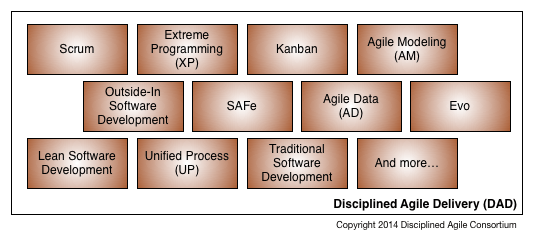
\includegraphics[scale=0.8]{hybrid1}
	\caption{DAD als hybrides Vorgehensmodell}
	\label{fig:hybrid}
\end{figure}
\subsection{Phasen in DAD}
Allgemein kann gesagt werden das DAD aus drei Phasen besteht Inception, Construction und Transition.\smallskip
\begin{figure}[H]
	\centering
	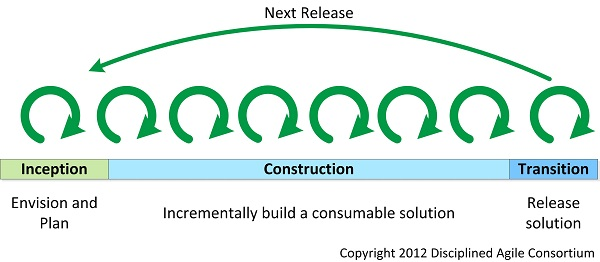
\includegraphics[width=\textwidth]{lifecycle}
	\caption{Highlevel Lifecycle von DAD}
	\label{fig:lifecycle}
\end{figure}\medskip
In der \textbf{Inception} Phase wird die Planung und Analyse des Projekts und dessen Ressourcen gemacht. Dies umfasst folgende Schritte:\smallskip
\begin{itemize}
	\item Initiales Team bilden
	\item Projekt Vision identifizieren
	\item Mit Stakeholder auf die Projekt Vision einigen
	\item Auf Unternehmensstrategie abstimmen
	\item Technische Strategie, initiale Anforderungen und initiale Release-Planung festlegen
	\item Arbeitsumfeld einrichten
	\item Finanzierung sichern
	\item Risiken identifizieren
\end{itemize}
\medskip
Die \textbf{Construction} Phase beinhaltet die eigentliche Entwicklung und das Testen, wo das entsprechende Vorgehensmodell eingesetzt wird.\smallskip
\begin{itemize}
	\item Eine verwendbare Lösung liefern
	\item Ändernde Bedürfnisse der Stakeholder adressieren 
	\item Näher an das einsetzbare Produkt herankommen
	\item Qualität verbessern oder auf höhere Qualität erarbeiten
	\item Architektur frühzeitig beweisen
	\item Arbeitsumfeld einrichten
\end{itemize}\medskip
Die \textbf{Transition} Phase betrifft Zieleinhaltung und Lieferung.
\begin{itemize}
	\item Einsatzfähigkeit der Lösung sicherstellen
	\item Empfangsbereitschaft der Stakeholder sicherstellen
	\item Lösung in produktive Umgebung liefern
\end{itemize}
